\solutionSection

\textbf{Декомпозиция задачи} \\
Для каждого кадра:
\begin{enumerate}
	\item Перевод цветного изображения в ч/б (состоит из "0" и "1")
	\item Распознавание метки ARTag
	\begin{enumerate}
		\item Нахождение углов многоугольника (до 8)
		\item если углов больше 4 - "достраиваем" срезанные углы
		\item Нахождение центра метки, он же - бит четности (parity bit)
		\item Нахождение ключевого бита (key bit)
		\item "Сборка" двоичного числа
		\item Сверка с битом четности
		\item Перевод в десятичную систему счисления
	\end{enumerate}
\end{enumerate}

\begin{figure}[h]
	\centering
	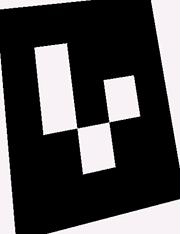
\includegraphics[width=0.4\linewidth]{2nd_tour/irs/03_Camera/03_ArTag_detecting/solution/03_artag_01.jpg}
	\caption{Исходное изображение метки ARTag}
	\label{fig:03_artag_01}
\end{figure}

\begin{figure}[h]
	\centering
	\includegraphics[width=0.4\linewidth]{2nd_tour/irs/03_Camera/03_ArTag_detecting/solution/03_artag_02.pdf}
	\caption{Изображение в ч/б варианте}
	\label{fig:03_artag_02}
\end{figure}

С алгоритмами перевода изображения в черно-белый вариант можно ознакомиться в презентации "Алгоритмические основы технического зрения" (\url{http://robolymp.ru/forum/index.php?PAGE_NAME=list&FID=116}).

Находим координаты углов n-угольника. В нашем случае получается 8-угольник:
% $A_1 (0, 52); A_2 (0, 10); A_3 (91, 0); A_4 (150, 0); A_5 (179, 168); A_6  (179, 198); A_7 (46, 233); A_8 (16, 233) $
\begin{figure}[H]
	\centering
	\includegraphics[width=0.6\linewidth]{2nd_tour/irs/03_Camera/03_ArTag_detecting/solution/03_artag_03.pdf}
	\caption{Координаты углов метки ARTag}
	\label{fig:03_artag_03}
\end{figure}

\begin{table}[H]
	\begin{center}
		\begin{tabular}{|c|c|c|c|c|c|c|c|c|}		
			\hline 
			& $A_1$ & $A_2$ & $A_3$ & $A_4$ & $A_5$ & $A_6$ & $A_7$ & $A_8$ \\ 
			\hline 
			X & 0 & 0 & 91 & 150 & 179 & 179 & 46 & 16 \\ 
			\hline 
			Y & 52 & 10 & 0 & 0 & 168 & 198 & 233 & 233 \\ 
			\hline 
		\end{tabular} 
		\caption{Координаты углов метки ARTag}
	\end{center}
\end{table}


Получается, что все 4 угла 'срезаны' значит нам надо их 'достроить'.

Каждый угол образуется пересечением отрезков близлежащих сторон метки. Например, $\angle$A (верхний левый) образуется пересечением отрезков $(A_1; A_8)$ и $(A_2; A_3)$, т.е. для нахождения координат угла нам достаточно найти точку пересечения прямых.

Исходя из линейной функции $y = k \cdot x + b$ найдем коэффициенты $k_{1,2}$ и $b_{1,2}$ для каждого отрезка:
\begin{equation*}
k=\frac{y_2-y_1}{x_2-x_1}; \qquad
b = y_2 - k \cdot x_2
\end{equation*}
Для отрезка ($A_1; A_8$):
\begin{equation*}
k_1=\frac{233-52}{16-0} = 11.31; \qquad
b_1 = 233 - 11.31 \cdot 16 = 52.04
%	\caption{Отрезок ($A_1; A_8$)}
\end{equation*}
Для отрезка ($A_2; A_3$):
\begin{equation*}
k_2 = \frac{0-10}{91-0} = -0.11; \qquad
b_2 = 0 + 0.11 \cdot 91 = 10.01
%	\caption{Отрезок ($A_1; A_8$)}
\end{equation*}
Теперь находим координаты $x; y$ $\angle$A:
\begin{equation*}
\begin{aligned}
x & = \frac{b_1-b_2}{k_2-k_1} =  \frac{52.04-10.01}{-0.11 - 11.31} = -3.68 \\
y &= k_1 \cdot x + b_1 = 11.31 \cdot -3.68 + 52.04 = 10.42 \\		
\end{aligned}
\end{equation*}
Аналогичным образом находим остальные углы и получаем координаты 4х угольника:\\

\begin{figure}[H]
	\centering
	\includegraphics[width=0.6\linewidth]{2nd_tour/irs/03_Camera/03_ArTag_detecting/solution/03_artag_04.pdf}
	\caption{Координаты полученного 4-х угольника}
	\label{fig:03_artag_04}
\end{figure}

Далее находим центр метки, он же будет "битом четности". В нашем случае центр метки - это точка пересечения диагоналей метки: $AC \cap BD$, в результате получаем координаты центра: $O(90; 104)$.

После чего находим центры сторон 4х-угольника: $AB$, $BC$, $CD$, $DA$. Для этого мы разделим отрезок каждой стороны на 2 равные части. Разберем на примере стороны $AB$:
\begin{equation*}
\begin{aligned}
x_{AB} & = \frac{x_1 + x_2}{2} = \frac{-4 + 149}{2} = 72.5 \\
y_{AB} & = \frac{y_1 + y_2}{2} = \frac{10 - 6}{2} = 2 \\		
\end{aligned}
\end{equation*}
Аналогичным способом находим координаты середин остальных сторон, в результате получаем (рис.\ref{fig:03_artag_05}).
\begin{figure}[H]
	\centering
	\includegraphics[width=0.6\linewidth]{2nd_tour/irs/03_Camera/03_ArTag_detecting/solution/03_artag_05.pdf}
	\caption{Разделение сторон периметра метки пополам}
	\label{fig:03_artag_05}
\end{figure}

\begin{table}[H]
	\begin{center}
		\begin{tabular}{|c|c|c|c|c|c|}
			\hline 
			& $O$ & $AB$ & $BC$ & $CD$ & $DA$\\
			\hline 
			X & 90 & 73 & 167 & 101 & 7 \\ 
			\hline 
			Y & 104 & -2 & 96 & 219 & 126 \\
			\hline 
		\end{tabular} 
		\caption{Координаты центра метки и середин сторон периметра метки}
	\end{center}
\end{table}

Теперь каждый отрезок от точки $O$ до точки на периметре 4х-угольника делим на 2.5 части. Почему на 2.5? В нашем случае маркер представляет квадрат из 5х5 клеток и центр находится в середине клетки, поэтому расстояние от центра метки до любой точки на краю метки составляет 2.5 клетки (рис. \ref{fig:03_artag_06}).
\\
\begin{figure}[H]
	\centering
	\includegraphics[width=0.6\linewidth]{2nd_tour/irs/03_Camera/03_ArTag_detecting/solution/03_artag_06.pdf}
	\caption{Полученные точки в центрах клеток}
	\label{fig:03_artag_06}
\end{figure}

По полученным точкам $OA_1$, $OB_1$, $OC_1$, $OD_1$ находим "ключевой бит", по которому определятся начало отсчета двоичного числа на метке. В нашем случае "ключевой бит" находится в точке $OA_1$.

По точкам $OAB_1$, $OBC_1$, $OCD_1$, $ODA_1$ составляем двоичный код. Старший разряд двоичного числа является самым верхним от расположения "ключевого бита". 
\\

Расположение информационных битов, в зависимости от "ключевого бита", показаны на рис. \ref{fig:03_artag_07} и \ref{fig:03_artag_08}.
\begin{figure}[H]
	\centering
	\includegraphics[width=0.3\linewidth]{2nd_tour/irs/03_Camera/03_ArTag_detecting/solution/03_artag_07.pdf}
	\label{fig:03_artag_07}
	\caption{Общая схема метки ARTag}
\end{figure}

\begin{figure}[H]
	\centering
	\includegraphics[width=0.3\linewidth]{2nd_tour/irs/03_Camera/03_ArTag_detecting/solution/03_artag_08.pdf}
	\label{fig:03_artag_08}
	\caption{Расположение битов для нашего примера}
\end{figure}

В нашем случае получается двоичное число: $0001$ \\
Сверяем двоичное число с "битом четности": если в двоичном числе количество "1" нечетное, значит "бит четности" должен быть равен "1", если же количество "1" в двоичном числе четное, то "бит четности" должен быть равен "0".

Если проверка на четность прошла успешно, то принимаем ответ как правильный, если проверка не прошла, значит обрабатываем следующий кадр.

В нашем случае проверка прошла успешно, значит переводим полученное число из двоичной системы в десятичную и принимаем как правильный ответ, получается: 1.

Если кадров несколько, то лучше все их распознать и сравнить полученные результаты.
\\

\textbf{Ответ: на метке закодировано число 1.}

\codeExample

\inputPythonSource
%\inputCPPSource
